Der Laborversuch wurde am Freitag, den 21. März 2025, durchgeführt und innerhalb von 90 Minuten abgeschlossen.
\subsection{Einleitung und Vorbereitung}
Vor Beginn des Experiments fand eine kurze Einführung in das Thema Scherversuche statt. Dabei wurden die theoretischen Grundlagen erläutert, um das Verständnis für das Versuchsprinzip zu gewährleisten.
Im Anschluss erfolgte eine Anweisung zur Nutzung der Messgeräte, begleitet von einer Erklärung zu den verwendeten Messproben und den zu erwartenden Versuchsergebnissen.
Die Einweisung und Anweisung wurden von Prof. Dr.-Ing. Aylin Bicakci oder dem Laborpersonal durchgeführt.
\subsection{Meilsteine}
\begin{itemize}
    \item Verständnis der Messgeräte – Kennenlernen und richtige Handhabung der Geräte.
    \item Unterscheidung verschiedener Brucharten – Erkennen und Klassifizieren von Bruchmechanismen.
    \item Kritische Analyse – Bewertung der unterschiedlichen Bruchformen basierend auf Messwerten.
    \item Methodik der Scherversuche – Anwendung und Verinnerlichung des Prüfverfahrens.
    \item Erstellung des Laborberichts – Dokumentation der Ergebnisse und Analyse der Versuchsdaten.
\end{itemize}
\subsection{Struktur der Arbeit}
Um das Experiment effizient durchführen zu können, haben wir verschiedene Aufgaben verteilt, um die Durchführung des Experiments optimal zu gestalten. Die folgende Abbildung zeigt die Aufgabenverteilung.
\begin{figure}[H]
    \centering
    \adjustbox{max width=\textwidth}{
    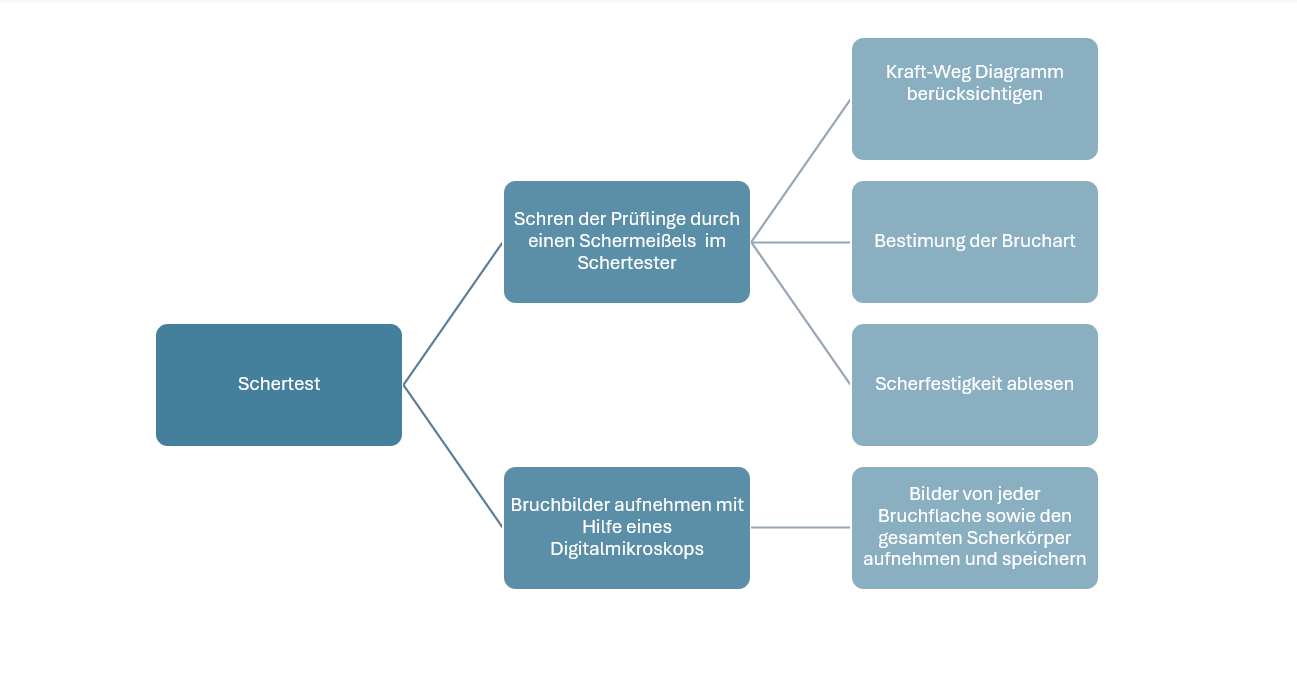
\includegraphics[scale=0.8]{Bilder/Struktur der Arbeit.png}}
    \caption{Darstellung des Strukturs der Arbeit}
    \label{Abb. :Darstellung des Strukturs der Arbeit}
\end{figure}
\subsection{Ausführung}
Nach der theoretischen Einführung begann der Versuch. Während der Versuchausführung wurden die Messwerte sorgfältig beobachtet, gespeichert und dokumentiert.
